\documentclass[aspectratio=169]{beamer}
\usepackage{../../LaTex/simplemetropolis} % Load your custom style
% % Input encoding.
\usepackage[utf8]{inputenc} % For accents in spanish: transforms "á" into "\'a"
\usepackage[T1]{fontenc} % Output encoding. Use to avoid silly problems on the output.
                         % See: http://tex.stackexchange.com/questions/664/why-should-i-use-usepackaget1fontenc
\usepackage{lmodern} % Latin Modern fonts have broader support
% AMS packages
\usepackage{amsmath}
\usepackage{amsfonts}
\usepackage{amssymb}
\usepackage{amsthm}
\usepackage{bbm}
% Other maths packages
\usepackage{mathtools}
\usepackage{leftindex}
% Tables
\usepackage{booktabs}  % For professional tables
\usepackage{multirow}  % For multirow formatting
% Include animated gifs
\usepackage{animate}
% Hyperlink
\usepackage{hyperref}
\hypersetup{
	final,
    bookmarksnumbered=true,
    bookmarksopen=true,
    bookmarksopenlevel=0,
    unicode=false,          % non-Latin characters in Acrobat?s bookmarks
    pdftoolbar=true,        % show Acrobat?s toolbar?
    pdfmenubar=true,        % show Acrobat?s menu?
    pdffitwindow=false,     % window fit to page when opened
    pdftitle={Quantitative Methods For Humanities},    % title
    pdfdisplaydoctitle=true, %display document title instead of file name in title bar
    pdftoolbar=true,
    pdfmenubar=true,
    pdflang={English},
    pdfauthor={Abel Guada Azze},     % author
    pdfsubject={Quantitative Methods For Humanities},   % subject of the document
    pdfcreator={Abel Guada Azze},   % creator of the document
    pdfproducer={Abel Guada Azze}, % producer of the document
    pdfkeywords={Quantitative Methods} {R}, % list of keywords
    pdfnewwindow=true,      % links in new window
    breaklinks=true,
    hidelinks,
    colorlinks,
    linkcolor=CUNEFOrange,          % color of internal links (change box color with linkbordercolor)
    citecolor=black,        % color of links to bibliography
    filecolor=cyan,      % color of file links
    urlcolor=magenta           % color of external links
}
% Import icons
\usepackage{fontawesome}
\usepackage{tikz}
% \pgfplotsset{compat=1.18}
% \usepackage{tkz-euclide}
\usetikzlibrary{shapes,arrows,matrix,positioning,calc}
\newcommand{\tikzmark}[1]{\tikz[baseline,remember picture] \coordinate (#1) {};}
% Define colors
\definecolor{amber}{rgb}{1.0, 0.49, 0.0} % Normalized RGB
\definecolor{firebrick3}{RGB}{207, 33, 32} % 8-bit RGB
\definecolor{deepskyblue3}{RGB}{0, 155, 206} % 8-bit RGB
\definecolor{darkorange3}{RGB}{206, 102, 0} % 8-bit RGB
\definecolor{darkolivegreen3}{RGB}{163, 207, 91} % 8-bit RGB
\definecolor{purpleR}{RGB}{160, 32, 240}
% Customizable new commands
\usepackage{xparse}
% Plain macros
\newcommand{\R}{\mathbb{R}} % real number set
\newcommand{\N}{\mathbb{N}} % natural number set
\newcommand{\lp}{\left(} % left parenthesis
\newcommand{\rp}{\right)} % right parenthesis
\newcommand{\lb}{\left[} % left brackets
\newcommand{\rb}{\right]} % right brackets
\newcommand{\lc}{\left\{} % left curly brackets
\newcommand{\rc}{\right\}} % right curly brackets
\newcommand{\la}{\langle} % left angled brackets
\newcommand{\ra}{\rangle} % right angled brackets
\newcommand*{\defeq}{\mathrel{\vcenter{
                     \baselineskip0.5ex\lineskiplimit0pt
                     \hbox{\scriptsize.}\hbox{\scriptsize.}
                     }}%
                     =}
                     \newcommand{\Rcoef}{\textsf{R}^2} % Coefficient of determination
\newcommand{\adjRcoef}{\oline{\textsf{R}}^2} % Coefficient of determination
\newcommand{\SER}{\textsf{SER}} % Standard error of the regression
\newcommand{\SSR}{\textsf{SSR}} % Sum of squared residuals
\newcommand{\ESS}{\textsf{ESS}} % explained sum of squares
\newcommand{\TSS}{\textsf{TSS}} % total sum of squareds
% Macros with arguments
\newcommand{\lrav}[1]{\left|#1\right|} % absolute value
\newcommand{\wtilde}[1]{\widetilde{#1}}
\newcommand{\what}[1]{\widehat{#1}}
\newcommand{\oline}[1]{\overline{#1}}
\newcommand{\bs}[1]{\boldsymbol{#1}}
\newcommand{\lrp}[1]{\lp#1\rp} % left-right parenthesis
\newcommand{\lrb}[1]{\lb#1\rb} % left-right brackets
\newcommand{\lrc}[1]{\lc#1\rc} % left-right curly brackets
\newcommand{\lra}[1]{\la#1\ra} % left-right angled brackets
\RenewDocumentCommand{\Pr}{oe{_^}}{% Probability P
  \operatorname{\mathbb{P}}%
  \IfValueT{#2}{_{#2}}%
  ^{\IfValueTF{#3}{#3}{}}%
  \IfValueT{#1}{\lp #1 \rp}%
}
\NewDocumentCommand{\Esp}{oe{_^}}{%
  \operatorname{\mathbb{E}}%
  \IfValueT{#2}{_{#2}}%
  ^{\IfValueTF{#3}{#3}{}}%
  \IfValueT{#1}{\lb #1 \rb}%
}
\newcommand{\Var}[1]{\mathbb{V}ar\lb #1\rb} % variance
\newcommand{\Cov}[2]{\mathbb{C}ov\lb #1, #2\rb} % covariance
% Title, subtitle, author, and date
\title{Quantitative Methods for Humanities}
\subtitle{Probability}
\author{}
\date{2025/2026}

\begin{document}

% Title page with custom background
{
    \usebackgroundtemplate{
\includegraphics[width=\paperwidth,height=\paperheight]{../../LaTex/img/title_page.png}}
    \begin{frame}[plain]
        % Logo in the upper left corner
        \vspace{-1cm} % Space between the logo and title
        {\hspace{-0.45cm} 
\includegraphics[width=2.5cm]{../../LaTex/img/logoCUNEF.png}} % Adjust the width as needed

        \vspace{1cm} % Space between the logo and title
        {\usebeamerfont{title}\usebeamercolor[fg]{title}\inserttitle\par}
        \vspace{-0.05cm} % Reduced space between title and separator
        \usebeamertemplate{title separator}
        \vspace{-0.05cm} % Reduced space between separator and subtitle
        {\usebeamerfont{subtitle}\usebeamercolor[fg]{subtitle}\insertsubtitle\par}
        \vfill
        {\usebeamerfont{date}\usebeamercolor[fg]{date}\insertdate\par}
    \end{frame}
}

% \begin{frame}{R Requirements}
%     \centering
%     Take the lessons PROBABILITY1 and PROBABILITY2 from the course \texttt{qss-swirl}
% \end{frame}

\section{\large Basic notions of Probability}

\begin{frame}{What is Probability?}
    \begin{itemize}
        \item \textbf{Measure of Uncertainty:} Quantifies how likely an event is to occur.
        \item \textbf{Examples.} How likely is:\\
        \begin{itemize}
            \item[$\bullet$] for Obama to win the 2008 US presidential election?
            \item[$\bullet$] for people living in a certain region to belong to a given racial group?
            \item[$\bullet$] to pass a quiz without studying, by answering at random? :)
            \item[$\bullet$] to suffer from a drug side effect?
        \end{itemize}
    \end{itemize}
\end{frame}

\begin{frame}{Frequentist Interpretation}
    \begin{itemize}
        \item \textbf{Definition:} Probability = Relative frequency in repeated experiments under identical conditions.
        \item \textbf{Example:} A fair coin lands heads $\approx 50\%$ over many tosses.
    \end{itemize}
    \vspace{0.5cm}
    \textbf{Challenges:}
    \begin{itemize}
        \item Experiments can’t always be repeated identically or infinitely.
        \item Social/political events (e.g., elections) don’t fit this framework.
    \end{itemize}
\end{frame}

\begin{frame}{Bayesian Interpretation}
    \begin{itemize}
        \item \textbf{Subjective Belief:} A measure of one's confidence about an event.
        \item Values range from 0 (impossible) to 1 (certain).
        \item \textbf{Example:} The probability of Obama winning in 2008 = X\%, reflects belief.
    \end{itemize}
    \vspace{0.3cm}

    \textbf{Frequentists vs Bayesians}
    \begin{itemize}
        \item \textbf{Frequentist:} Objective, based on repeatable experiments.
        \item \textbf{Bayesian:} Subjective, based on individual belief and prior knowledge.
    \end{itemize}
    \vspace{0.3cm}
    
    \textbf{Critiques and Counterpoints}
    \begin{itemize}
        \item \textbf{Critics:} Subjectivity hinders scientific consensus.
        \item \textbf{Bayesians:} Recognizing subjectivity makes science more honest.
    \end{itemize}

\end{frame}

\section{\large Definitions and axioms}

\begin{frame}{Unified Mathematical Foundation}

    Despite the apparent discrepancies between Frequenstist and Bayesians, 
    \begin{itemize}
        \item both frameworks share the same mathematical rules;
        \item they are unified in the common Theory of Probability, developed by Andrey Kolmogorov in 1933;
        \item differences are only interpretative.
    \end{itemize}
    
\end{frame}

\begin{frame}{Basic concepts}
    \begin{itemize}
        \item \textbf{Experiment:} An action or set of actions producing stochastic events of interest.
        \item \textbf{Sample Space (\(S\)):} The set of all possible outcomes of an experiment.
        \item \textbf{Event:} A subset of the sample space.
    \end{itemize}
    \vspace{0.5cm}
    Examples:
    \begin{itemize}
        \item Flipping a coin: \(S = \{ \text{Heads, Tails} \}\)
        \item US Presidential Election: \(S = \{ \text{Obama wins, McCain wins, Third-party wins} \}\)
    \end{itemize}
\end{frame}

\begin{frame}{Probability Axioms}
    \begin{enumerate}
        \item \textbf{Non-negativity:} \(P(A) \geq 0\)
        \item \textbf{Normalization:} \(P(S) = 1\)
        \item \textbf{Addition Rule (Mutually Exclusive Events):} \(P(A \text{ or } B) = P(A) + P(B)\) if $A\cap B = \emptyset$.
    \end{enumerate}
    \vspace{0.5cm}
    Example of mutually exclusive events:
    \begin{itemize}
        \item Event \(A\): Obama wins
        \item Event \(B\): McCain wins
        \item There is no third party
        \item \(P(A \text{ or } B) = P(A) + P(B)\)
    \end{itemize}
\end{frame}

\begin{frame}{General Addition Rule}
    For events \(A\) and \(B\) (not mutually exclusive):
    \[
    P(A \text{ or } B) = P(A) + P(B) - P(A \text{ and } B)
    \]
    \vspace{0.5cm}
    \textbf{Example:}
    \begin{itemize}
        \item Event \(A\): Obama wins
        \item Event \(B\): McCain wins
        \item There is a third party
        \item \(P(A \text{ or } B) = P(A) + P(B) - P(A \text{ and } B)\)
    \end{itemize}
\end{frame}

\begin{frame}{Complement Rule and Total Probability}
    \begin{itemize}
        \item \textbf{Complement Rule:} \(P(A^c) = 1 - P(A)\)
        \item \textbf{Law of Total Probability:} \(P(A) = P(A \text{ and } B) + P(A \text{ and } B^c)\)
    \end{itemize}
    \vspace{0.5cm}
    \textbf{Example:}
    \begin{itemize}
        \item \(P(A^c)\): Probability of not \(A\)
        \item \(P(A)\): Decomposed into contributions from \(B\) and \(B^c\)
    \end{itemize}
\end{frame}

\section{\large Counting to compute probability}

\begin{frame}{Definition of Probability by Counting}
    For equally likely outcomes, the probability of an event \(A\) is:
    \[
    P(A) = \frac{\text{Number of elements in } A}{\text{Number of elements in } S}
    \]
    Example:
    \begin{itemize}
        \item Tossing a fair coin 3 times: \(S = \{HHH, HHT, HTH, HTT, THH, THT, TTH, TTT\}\)
        \item Event \(A\): Landing on heads at least twice \(A = \{HHH, HHT, HTH, THH\}\)
        \item \(P(A) = \frac{4}{8} = 0.5\)
    \end{itemize}
\end{frame}

\begin{frame}{Permutations}
    \begin{itemize}
        \item \textbf{Permutations:} The number of ways to arrange \(k\) objects out of \(n\) unique objects.
        \item \textbf{Example:}
        \begin{itemize}
            \item[$\bullet$] How to arrange $2$ objects out of $3$ unique objects?
            \item[$\bullet$] Objects: \(A, B, C\)
            \item[$\bullet$] Arrangements: \(\{AB, AC, BA, BC, CA, CB\}\)
            \item[$\bullet$] Total number of arrangements: \(3! = 3 \times 2 \times 1 = 6\)
        \end{itemize}
        \item \textbf{General formula:} $\leftindex_{n}{P}_k = \frac{n!}{(n-k)!}$
        \begin{itemize}
            \item[$\bullet$] $n!$ is the factorial of \(n\), defined as \(n! = n \times (n-1) \times \cdots \times 1\)
        \end{itemize}
    \end{itemize}
\end{frame}

\begin{frame}{The Birthday Problem}
    \begin{itemize}
        \item \textbf{Question:} How large should a group be so that the probability of at least two people in the group sharing the same birthday exceeds 0.5?
        \item \textbf{Key Idea:}
        \[
        P(\text{at least two people have the same birthday}) = 1 - P(\text{nobody shares a birthday})
        \]
        \item \textbf{Formula for \(P(\text{nobody shares a birthday})\)}
        \[
        P(\text{nobody shares a birthday}) = \frac{_{365}P_k}{365^k} = \frac{365!}{365^k (365-k)!}
        \]
        \item \textbf{How to compute?} $365!$ and $365^k$ are large numbers. Try to compute them in your calculator
        \item \textbf{The log solution:} Work in logarithmic scale (products transform into sums) and then exponentiate back to the original scale
        \item \textbf{in R:} \texttt{lfactorial} \\
        \scriptsize{Up to +0.2 points for the first student posting in the forum a piece of code with a function to compute the probability asked, provided the number of people}
    \end{itemize}
    
\end{frame}

\begin{frame}{Solution to the Birthday Problem}
    \vspace{0.2cm}
    \centering
    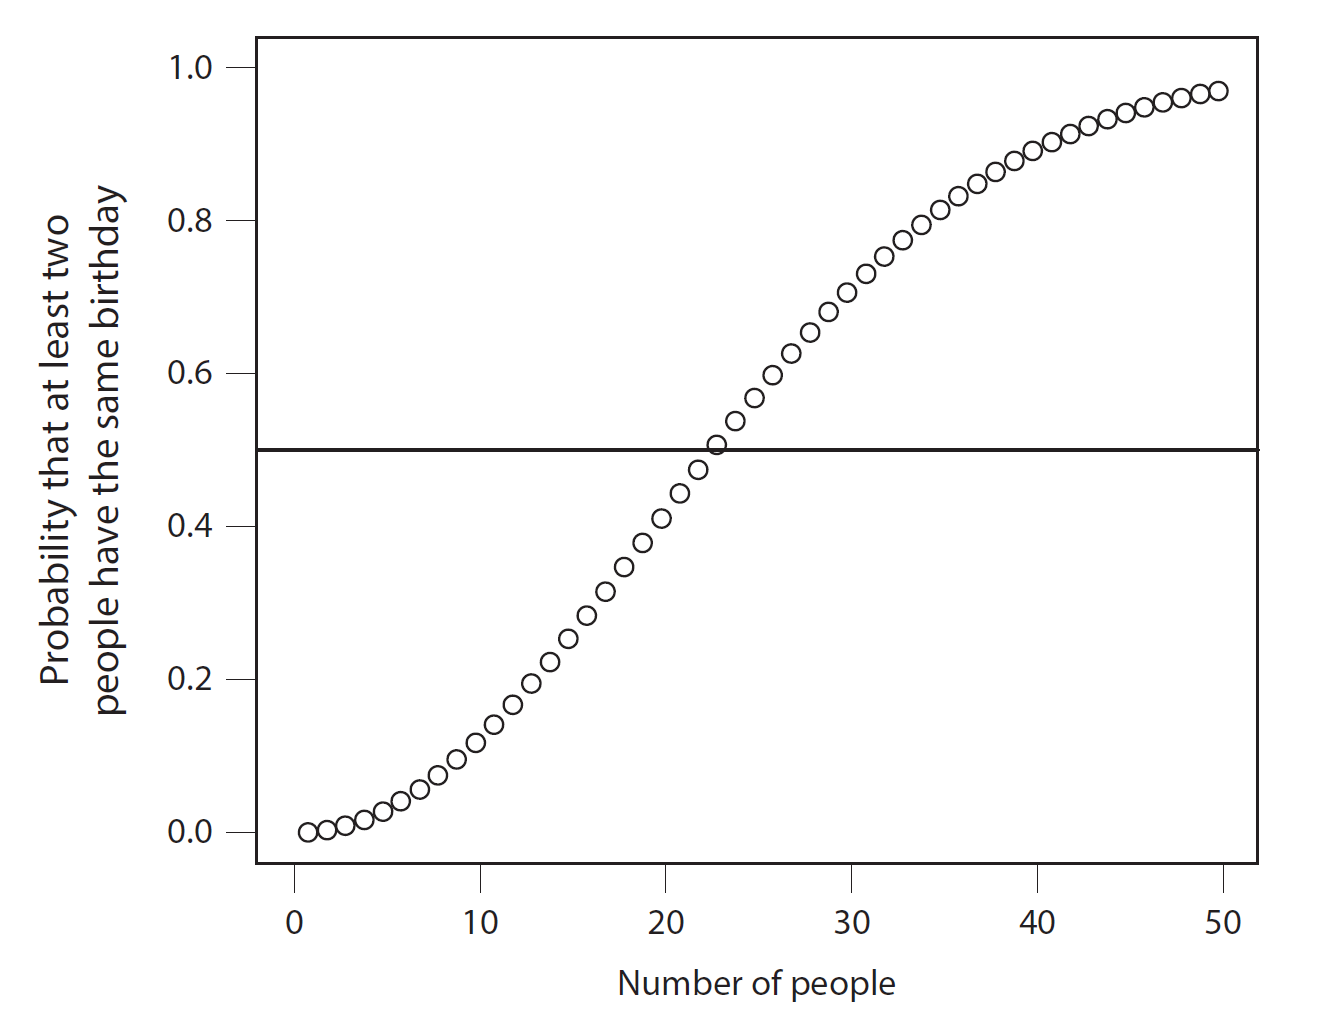
\includegraphics[scale=0.25]{../../LaTex/img/birthday_problem_plot.png} 
\end{frame}

\begin{frame}{Combinations}
    \begin{itemize}
        \item \textbf{Combinations:} Ways to choose \(k\) distinct objects from \(n\) elements \textbf{without considering order}.
        \item \textbf{Difference from permutations:} Order does not matter.
        \item \textbf{Example:}
        \begin{itemize}
            \item \textbf{Objects:} \(A, B, C\)
            \item \textbf{Permutations (order matters):} \(AB, BA, AC, CA, BC, CB\) \(\Rightarrow 6\)
            \item \textbf{Combinations (order doesn't matter):} \(AB, AC, BC\) \(\Rightarrow 3\)
        \end{itemize}
        \item \textbf{General formula:} $_nC_k = \binom{n}{k} = \frac{n!}{k!(n-k)!}$
    \end{itemize}
\end{frame}

\begin{frame}{Example: probability of choosing at least 2 women in the committee}
    \textbf{Problem:} Suppose that we are creating a committee of 5 out of 20 people (10 men and 10 women). Each person is equally likely to be assigned to the committee. What is the probability that at least 2 women are on the committee?
    
    \vspace{0.5cm}
    \textbf{Solution:}
    \begin{itemize}
        \item Use the complement event and the additivity of the probability for disjoint sets:
        $$
        P(\text{at least 2 women}) = 1 - P(\text{no woman}) - P(\text{exactly 1 woman})
        $$
        \item \textbf{Total ways to form a committee of 5 from 20:} $\binom{20}{5} = 15,504$
        \item \textbf{Total ways to choose no woman (5 men):} $\binom{10}{5} = 252$
        \item \textbf{Total Ways to choose exactly 1 woman:} $\binom{10}{1} = 2100$
        \item \textbf{Compute probability:}
        $$
        P(\text{at least 2 women}) = 1 - \frac{252}{15,504} - \frac{2,100}{15,504} = 0.84.
        $$
    \end{itemize}
\end{frame}

\begin{frame}{Example. Acrostic by change?}

    \hspace{0.45cm} \textbf{California Governor Arnold Schwarzenegger’s Veto Message in 2009.}
    \vspace{-0.1cm}
    
    \begin{center}
        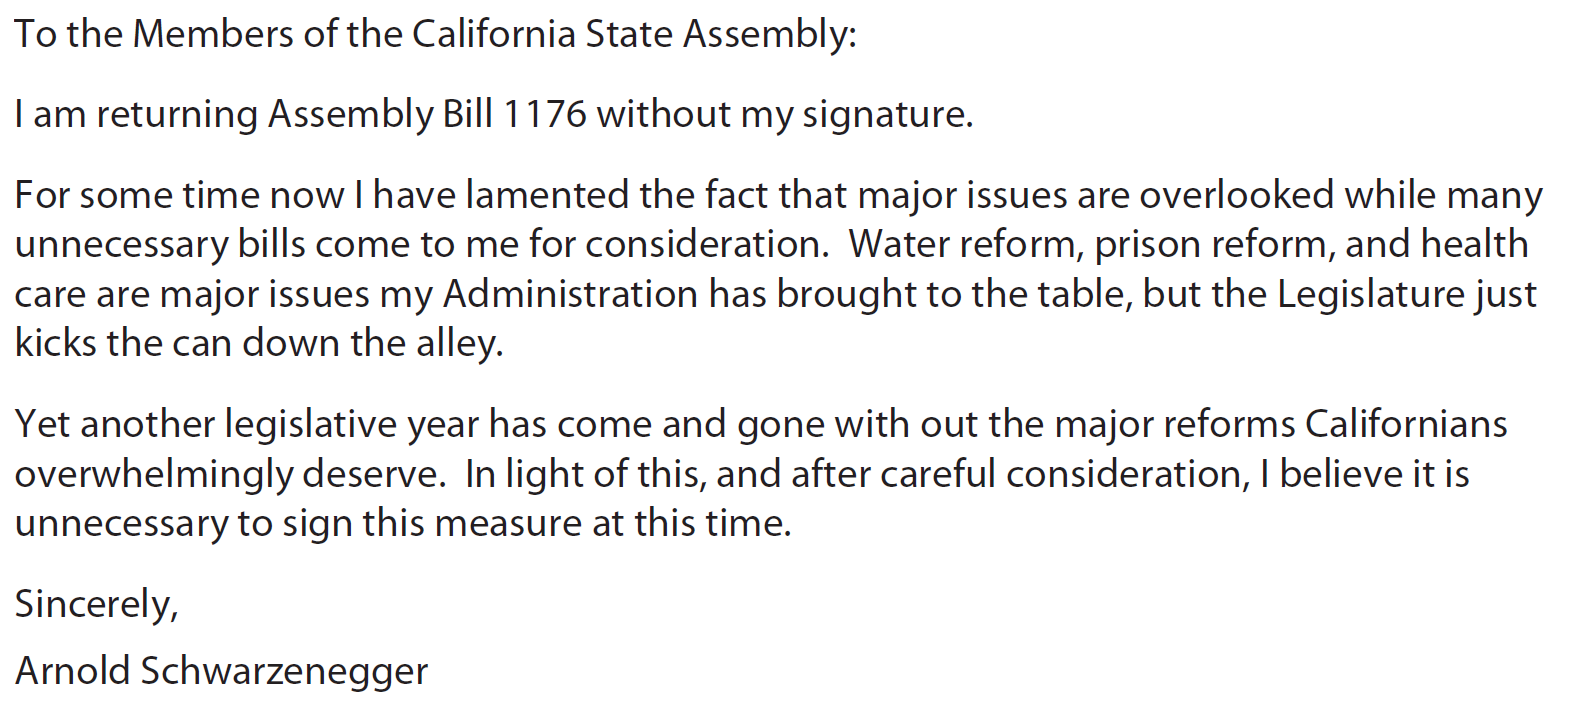
\includegraphics[height=4.8cm, width=14cm]{../../LaTex/img/Arnol_message.png}
    \end{center}
    \vspace{-0.2cm}
    
    \begin{itemize}
        \item \textbf{Question:} Was the ``Fuck you'' acrostic intentional?
        \item \textbf{Schwarzenegger’s reply:} ``My goodness. What a coincidence. I suppose when you do so many vetoes, something like this is bound to happen.''
    \end{itemize}
    
\end{frame}

\begin{frame}{Solution to the Veto Message Problem}

    \begin{itemize}
    \item The possible line breaks for each given letter are as follows:
    \begin{itemize}
        \item[$\bullet$] "u" has \textbf{1} possible break (in "unnecessary").
        \item[$\bullet$] "c" has \textbf{3} possible breaks (in "come," "consideration," "care").
        \item[$\bullet$] "k" has \textbf{1} possible break (in "kicks").
        \item[$\bullet$] "y" has \textbf{2} possible breaks (in "Yet," "year").
        \item[$\bullet$] "o" has \textbf{2} possible breaks (in "overwhelmingly," "of").
        \item[$\bullet$] "u" again has \textbf{1} possible break (in "unnecessary").
    \end{itemize}
    
    \item Multiplying these possibilities:
    \[
    1 \times 3 \times 1 \times 2 \times 2 \times 1 = 12
    \]
    
    \item Thus, there are \textbf{12 different ways} to create these line breaks.
    \end{itemize}
    
\end{frame}

\begin{frame}{Solution to the Veto Message Problem}
    
    \begin{itemize}
        
        \item Total number of ways to insert 6 line breaks into 85 words (\texttt{choose(84, 6)} in R):
        \[
        \binom{84}{6} = \frac{84!}{6! \cdot 78!} \approx 406,481,544
        \]
        
        \item \textbf{Probability:}
        \[
        P = \frac{12}{\binom{84}{6}} \approx \frac{12}{406,481,544} \approx 1 \text{ in } 34 \, \text{million}
        \]
        
        \item \textbf{Conclusion:} The acrostic was an extremely unlikely event.
    \end{itemize}
    
\end{frame}

% \section{\large Sampling and simulations}

% \begin{frame}{What is Sampling?}
%     \begin{itemize}
%         \item \textbf{Sampling with Replacement:}
%         \begin{itemize}
%             \item Each element can be selected multiple times.
%             \item Example: Simulating birthdays where each day of the year is equally likely for every person.
%         \end{itemize}
%         \item \textbf{Sampling without Replacement:}
%         \begin{itemize}
%             \item Each element can be selected only once.
%             \item Example: Selecting respondents in a simple random sample (SRS) for surveys.
%         \end{itemize}
%     \end{itemize}
% \end{frame}

% \begin{frame}{Monte Carlo Simulation Method}
%     \begin{itemize}
%         \item A stochastic method to approximate solutions by randomly generating quantities of interest.
%         \item Steps:
%         \begin{enumerate}
%             \item Define the problem (e.g., probability of shared birthdays).
%             \item Simulate the process (e.g., draw birthdays for \(k\) people).
%             \item Repeat simulations (\(n\) times) and compute the fraction of desired outcomes.
%         \end{enumerate}
%         \item Example: Birthday problem
%         \begin{itemize}
%             \item Simulation estimate: \(P(\text{at least two shared birthdays}) \approx 0.509\).
%             \item Analytical solution: \(P \approx 0.507\).
%         \end{itemize}
%     \end{itemize}
% \end{frame}

% \begin{frame}{Advantages and Limitations of Simulations}
%     \textbf{Advantages:}
%     \begin{itemize}
%         \item Intuitive: Emulates real-world data generation processes.
%         \item Flexible: Applies to problems without closed-form analytical solutions.
%     \end{itemize}
%     \vspace{0.5cm}
%     \textbf{Limitations:}
%     \begin{itemize}
%         \item Monte Carlo Error: Estimates vary due to randomness.
%         \item Reducing error requires increasing the number of simulations.
%     \end{itemize}
%     \textbf{Note:} Simulation with 1,000,000 trials yields \(P \approx 0.508\), closer to the true value.
% \end{frame}


\section{\large Conditional, Marginal, Joint Probabilities, and Independence}

\begin{frame}{Conditional probability as a way to update our believes}
    
    % \textbf{Why is Conditional Probability Important?}
    
    \begin{itemize}
        \item Conditional probability allows us to \textbf{update our beliefs about the likelihood of an event based on new information.}
        \item It refines our predictions by incorporating relevant evidence, making probability assessments more accurate.
        \item \textbf{Bayes' Theorem} is a fundamental tool that uses conditional probability to update beliefs and make informed decisions.
    \end{itemize}
    
    % \textbf{Key Takeaway:} 
    % \begin{itemize}
    %     \item The more relevant information we have, the better we can estimate the true likelihood of an event occurring.
    % \end{itemize}
    \vspace{0.3cm}
    
    \begin{center}
        \begin{tcolorbox}[enhanced,sharp corners,
            width=7.3cm,
            colback=white,
            overlay={
                % Upper left corner (quotation mark)
                \node[anchor=north west,fill=white,draw=white,circle,inner sep=1pt] 
                at ([xshift=-0.17cm,yshift=0.2cm]frame.north west) {\faQuoteLeft};
                % Lower right corner (quotation mark)
                \node[anchor=south east,fill=white,draw=white,circle,inner sep=1pt] 
                at ([xshift=0.17cm,yshift=-0.2cm]frame.south east) {\faQuoteRight};
            }
            ]
            How can we live if we don’t change?
            \vspace{0cm}
            
            {\small - Beyoncé. Lyric from “Satellites.”}
        \end{tcolorbox}
    \end{center}
        
\end{frame}

\begin{frame}{Our brains use conditional probability all the time. Example 1}
    
    \textbf{Example: Checking the Weather Before Going Outside.} \\
    Suppose you’re about to leave your house, and you quickly glance out the window to check the weather.
    \vspace{0.3cm}
    
    \begin{itemize}
        \item \textbf{Initial Belief:} You checked the forecast earlier, and it said there was a 30\% chance of rain.
        \item \textbf{New Information:} You now see dark clouds forming and feel a sudden drop in temperature.
        \item \textbf{Refined Prediction:} Your brain updates the probability of rain, now considering it much higher. You grab an umbrella before heading out.
    \end{itemize}
    \vspace{0.3cm}
    
    Even without formal calculations, your brain is constantly updating expectations based on incoming information, just like conditional probability!
\end{frame}

\begin{frame}{Our brains use conditional probability all the time. Example 2}
    
    \textbf{Example:} You are meeting a friend for coffee, and before you arrive, you wonder what mood she will be in.
    \vspace{0.3cm}
    
    \begin{itemize}
        \item \textbf{Initial Belief:} You have a general idea of your friend's mood based on past experiences.
        \item \textbf{New Information:} When you meet her she is smiling and speaking energetically.
        \item \textbf{Refined Prediction:} You update your belief that she is likely to be in a good mood.
    \end{itemize}
    \vspace{0.3cm}
    
    Even without formal calculations, your brain is constantly updating expectations based on incoming information, just like conditional probability!
\end{frame}

\begin{frame}{Definitions}
    \begin{itemize}
        \item \textbf{Conditional Probability:} The probability of event \(A\) given \(B\) has occurred.
        \[
        P(A | B) = P(A \text{ and } B)/P(B)
        \]
        \item \textbf{Joint Probability:} The probability of two (or more) events occurring together.
        \[
        P(A \text{ and } B) = P(A \cap B)
        \]
        \item \textbf{Marginal Probability\footnote{\scriptsize{The concept of marginal probability implies that some joint probability has been considered previously}}:} The probability of a single event occurring.
        \[
        P(B)
        \]
    \end{itemize}
\end{frame}

\begin{frame}{Conditional probability. Problem}

    \textbf{Scenario:} Consider two couples expecting twins. One couple had an ultrasound and determined that at least one twin is a boy. The other couple found out at delivery that the first-born is a boy. What is the probability that both twins are boys in each case?
    \vspace{0.3cm}
    
    \textbf{Solution:}
    \begin{itemize}
        \item The sample space for the twins' genders is: \[ \Omega = \{ GG, GB, BG, BB \} \]
        \item \textbf{Couple 1: knowing at least one twin is a boy}
        \begin{align*}
            P(BB | \text{at least one boy}) &= \frac{P(BB)}{P(BB \cup BG \cup GB)} 
            = \frac{1/4}{3/4} = \frac{1}{3}.
        \end{align*}
        \item \textbf{Couple 2: knowing the elder twin is a boy}
        \begin{align*}
            P(BB | \text{elder twin is a boy}) &= \frac{P(BB)}{P(BB \cup BG)} 
            = \frac{1/4}{1/2} = \frac{1}{2}.
        \end{align*}
    \end{itemize}
        
    \textbf{Conclusion:} The information upon we condition matters.
\end{frame}

\begin{frame}{Law of Total Probability}
    \begin{coolblock}{Law of Total Probability}
    The (marginal) probability of an event \(A\) can be computed using all possible scenarios \(B_i\):
    \[
    P(A) = \sum_{i} P(A \cap B_i) = \sum_{i} P(A | B_i)P(B_i)
    \]
    \end{coolblock}
    \vspace{0.3cm}
    
    \textbf{Example: Probability of fake news} \\
    In an online journal, the probability of an article being classified as ``fake news'' ($FN$) is $0.29$ if its title contains exclamation marks ($E$), and $0.11$ if it does not. If 16\% of the articles contain exclamation marks, what is the probability of an article being classified as ``fake news''?
    \vspace{0.2cm}
    
    \textbf{Solution:} 
    \vspace{-0.4cm}
    \begin{align*}
        P(FN) &= P(FN\ |\ E)P(E) + P(FN\ |\ E^c)P(E^c) \\
        &= 0.29\times0.16 + 0.11\times0.84 = 0.1388    
    \end{align*}
    
\end{frame}

\begin{frame}{Independence}
    \begin{itemize}
        \item Events \(A\) and \(B\) are \textbf{independent} if knowing \(B\) gives no additional information about \(A\):
        \[
        P(A | B) = P(A) \quad \text{and} \quad P(B | A) = P(B)
        \]
        \item Equivalent Definition:
        \[
        P(A \text{ and } B) = P(A)P(B)
        \]
    \end{itemize}

\end{frame}

\begin{frame}{The Monty Hall Problem}
    \textbf{Problem Setup:}
    \begin{itemize}
        \item Choose one of three doors:
            \begin{itemize}
                \item[$\bullet$] One door conceals a car (win).
                \item[$\bullet$] Two doors conceal goats (lose).
            \end{itemize}
        \item Monty opens a door with a goat and offers you the chance to switch.
        \item \textbf{Question:} Should you switch or stay to maximize your chance of winning?
    \end{itemize}
\end{frame}

\begin{frame}{Solution of the Monty Hall problem. Intuition}
    
    \begin{itemize}
        \item \textbf{Common (mistaken) belief:} ``Now I have fifty-fifty of winning, so why changing?''
        \item \textbf{You don't have ``fifty-fifty'':} 
        \begin{itemize}
            \item[$\bullet$] \textbf{If you don't change your original choice:} \\
            When your choice was made you had one-in-three probability of winning. If you stick to your original election, revealing a door does not change that probability.
            $$
            P(\text{car}\ |\ \text{do not switch}) = 1/3
            $$
            \item[$\bullet$] \textbf{If you change your original choice:} \\ 
            In this case you would win the car whenever you would have been mistaken, which has two-in-three probability of occur.
            $$
            P(\text{car}\ |\ \text{switch}) = 2/3
            $$
        \end{itemize}
        % \item 
        % \item \textbf{Switching increases your changes:}
        % \begin{itemize}
        %     \item[$\bullet$] If your first choice is a goat (\(P = \frac{2}{3}\)), switching always leads to the car.
        %     \item[$\bullet$] If your first choice is the car (\(P = \frac{1}{3}\)), switching loses.
        % \end{itemize}
    \end{itemize}
    \vspace{0.2cm}

    \begin{center}
        See a more intuitive explanation \href{https://www.youtube.com/watch?v=DlphpbxNTLw}{here}.
    \end{center}
\end{frame}

\begin{frame}{Solution of the Monty Hall problem. Law of total probability}
    
    \begin{itemize}
        \item Probability of winning if you:
        \begin{itemize}
            \item[$\bullet$] \textbf{Do not switch:}
            \begin{align*}
                P(\text{car}) &= P(\text{car} \mid \text{car first}) P(\text{car first}) + P(\text{car} \mid \text{goat first}) P(\text{goat first}) \\
                &= P(\text{car first}) = \frac{1}{3}.
            \end{align*}
            % P(\text{Car | Initial choice}) = 
            % \frac{1}{3}
            % \]
            \item[$\bullet$] \textbf{Switch:}
            \begin{align*}
                P(\text{car}) &= P(\text{car} \mid \text{car first}) P(\text{car first}) + P(\text{car} \mid \text{goat first}) P(\text{goat first}) \\
                &= P(\text{goat first}) = \frac{2}{3}.
            \end{align*}
            % \[
            % P(\text{Car | Switch}) = \frac{2}{3}
            % \]
        \end{itemize}
    \end{itemize}
    
    \begin{itemize}
        \item \textbf{Not independence between winning and changing your mind:} The event ``wining the car'' is not independent to the event ``switching the door''.
    \end{itemize}
    \vspace{0.2cm}
    
    \scriptsize{Up to +0.2 points for the first student posting in the forum a piece of code with a function that computes the probabilities of winning and losing of the Monty Hall problem based on simulations}

\end{frame}

\section{\large Bayes's rule}

\begin{frame}{Bayes' Rule: Definition}
    \begin{coolblock}{Bayes' Rule}
    \[
    P(A | B) = \frac{P(B | A)P(A)}{P(B)}
    \]
    \end{coolblock}
    \begin{itemize}
        \item \(P(A)\): Prior probability (initial belief).
        \item \(P(A | B)\): Posterior probability (updated belief after observing \(B\)).
        \item \(P(B | A)\): Likelihood of observing \(B\) given \(A\).
        \item \(P(B)\): Marginal probability of \(B\).
    \end{itemize}
\end{frame}

\begin{frame}{Example: Economic Recession Forecast}
    Consider the following economic forecasting problem:
    \begin{itemize}
        \item Historically, there is a 1 in 20 chance that the economy will enter a Recession (R) in any given year.
        \item An economic indicator categorizes the economy of the current year as \textbf{High-Risk (HR)} for recession.
        \item Out of 100 years with a recession, 80 will be identified as high-risk by the indicator, and 20 will not be detected.
        \item There is a 1 in 10 chance that the economy is not in recession but the indicator still signals high-risk.
    \end{itemize}
    Given the result of the economic indicator, what is the probability that the economy will enter a recession?
\end{frame}

\begin{frame}{Economic Recession Forecast}
    \textbf{Problem:}
    \begin{itemize}
        \item Probability of a recession \(P(\text{R}) = 1/20 = 0.05\).
        \item Economic indicator is high-risk (HR) with:
        \begin{itemize}
            \item[$\bullet$] True positive rate $P(HR | R)= 0.80$,
            \item[$\bullet$] False positive rate $P(HR | R^c) = 0.10$.
        \end{itemize}
    \end{itemize}

    \textbf{Bayes' Rule:}
    $$
    P(R | HR) = \frac{P(HR | R) \cdot P(R)}{P(HR | R) \cdot P(R) + P(HR | R^c) \cdot P(R^c)}
    $$

    \textbf{Result:}
    $$
    P(R | HR) = \frac{0.80 \cdot 0.05}{0.80 \cdot 0.05 + 0.10 \cdot 0.95} \approx 0.297 \;\; (29.7\%)
    $$
\end{frame}

% \begin{frame}{Revisiting the Monty Hall problem}

%     We can use Bayes’ rule to solve the Monty Hall problem.
%     \begin{itemize}
%         \item Let $Di$, $D2$ and $D3$ represent the event that the first, second and third door has a car behind it, respectively, while the others have goats.
%         \item Since each door is equally likely to have a car behind it: 
%         \( P(D1) = P(D2) = P(D3) = 1/3 \)
%         \item Suppose we choose the first door and let $MC$ represent the event that Monty opens the third door.
%     \end{itemize}
%     We want to determine whether switching to the second door increases the probability of winning the car.

%     \textbf{Conditional Probabilities:}
%     \begin{itemize}
%         \item $P(MC\ |\ D1) = \frac{1}{2}$ (Monty chooses randomly between doors 2 and 3).
%         \item $P(MC\ |\ D2) = 1$ (Monty must open door 3 since door 2 has the car).
%         \item $P(MC\ |\ D3) = 0$ (Monty cannot open door 3 because it has the car).
%     \end{itemize}
    
% \end{frame}

% \begin{frame}{Policy Implications}
%     \textbf{High-Risk Indicator (\(P(\text{Recession | HR}) \approx 29.7\%\)):}
%     \begin{itemize}
%         \item Implement preemptive fiscal or monetary policies to mitigate risk.
%         \item Prepare stakeholders for potential challenges.
%     \end{itemize}

%     \textbf{Negative Indicator (\(P(\text{Recession | Not HR}) \approx 1.1\%\)):}
%     \begin{itemize}
%         \item Maintain current economic policies.
%         \item Reassure public and investors of stability.
%     \end{itemize}

%     \textbf{Conclusion:} Bayes' Rule helps decision-makers respond effectively to economic signals.
% \end{frame}

% \begin{frame}{Example: Medical Test for Down Syndrome}
%     Consider the following first-trimester screening test problem:
%     \begin{itemize}
%         \item A 35-year-old pregnant woman is told that 1 in 378 women of her age will have a baby with Down syndrome (DS).
%         \item A first-trimester ultrasound screening procedure indicates that she is in a hig-hrisk (HR) category.
%         \item Of 100 cases of DS, 86 mothers will receive a high-risk result and 14 cases of DS will be missed.
%         \item There is a 1 in 20 chance for a normal pregnancy to be diagnosed as high risk.
%     \end{itemize}   
%     Given the result of the screening procedure, what is the probability that her baby has DS? What would the probability be if the result had been negative?
% \end{frame}


% \begin{frame}{Example: Medical Test for Down Syndrome}
%     \textbf{Scenario:}
%     \begin{itemize}
%         \item Probability of Down Syndrome (\(P(\text{DS})\)): \(1/378 \approx 0.003\).
%         \item Test true positive rate (\(P(\text{HR | DS})\)): \(0.86\).
%         \item Test false positive rate (\(P(\text{HR | Not DS})\)): \(0.05\).
%     \end{itemize}
%     \textbf{Posterior Probability:}
%     \[
%     P(\text{DS | HR}) = \frac{P(\text{HR | DS})P(\text{DS})}{P(\text{HR | DS})P(\text{DS}) + P(\text{HR | Not DS})P(\text{Not DS})}
%     \]
%     Substituting values:
%     \[
%     P(\text{DS | HR}) = \frac{0.86 \times 0.003}{0.86 \times 0.003 + 0.05 \times 0.997} \approx 0.04
%     \]
%     \textbf{Conclusion:} Even with a high-risk result, the chance of Down Syndrome is small due to its rarity.
% \end{frame}

\section{\large Random variables}

\begin{frame}{What is a Random Variable?}
    \begin{itemize}
        \item A random variable assigns a numeric value to each event in the sample space. That is,
        $$
        X:S\rightarrow \R.
        $$
        \item Values must represent:
        \begin{itemize}
            \item[$\bullet$] \textbf{Mutually exclusive events:} No overlap between values.
            \item[$\bullet$] \textbf{Exhaustive events:} All events are represented.
        \end{itemize}
        \item Examples:
        \begin{itemize}
            \item[$\bullet$] Coin flip: Heads = 1, Tails = 0.
            \item[$\bullet$] Racial group: Black = 1, White = 2, Hispanic = 3, etc.
        \end{itemize}
    \end{itemize}
\end{frame}

\begin{frame}{Types of Random Variables}
    \begin{itemize}
        \item \textbf{Discrete Random Variable:}
        \begin{itemize}
            \item[$\bullet$] Takes a finite or countably infinite set of values.
            \item[$\bullet$] Examples: Number of years of education, racial group.
        \end{itemize}
        \item \textbf{Continuous Random Variable:}
        \begin{itemize}
            \item[$\bullet$] Takes any value within an interval of the real line.
            \item[$\bullet$] Examples: Height, weight, GDP.
        \end{itemize}
    \end{itemize}
\end{frame}

\begin{frame}{Mass, density, and distribution}
    \begin{itemize}
        \item \textbf{Probability Mass Function (PMF):}
        \begin{itemize}
            \item[$\bullet$] Defines the probability for discrete random variables to take a single value.
            \item[$\bullet$] \textbf{Definition:} \(f(x) = P(X = x)\).
        \end{itemize}
        \item \textbf{Probability Density Function (PDF):}
        \begin{itemize}
            \item[$\bullet$] Defines the likelihood for continuous random variables.
            \item[$\bullet$] It is a \textbf{positive function whose total area under the curve equals 1}, that is
            $$
            f(x) \geq 0,\quad \int_{\R}f(x)\, \mathrm{d}x = 1.
            $$
        \end{itemize}
        \item \textbf{Cumulative Distribution Function (CDF):}
        \begin{itemize}
            \item[$\bullet$] Represents the probability that a random variable is less than or equal to a value \(x\).
            \item[$\bullet$] \textbf{Formula:}
            $$
            F(x) = P(X \leq x) =
            \begin{cases}
                \sum_{k \leq x} f(k) & \text{(discrete)} \\
                \int_{-\infty}^x f(t) \, dt & \text{(continuous)}
            \end{cases}
            $$
        \end{itemize}
    \end{itemize}
\end{frame}

\begin{frame}{Bernoulli Distribution. The simplest discrete distribution}
    \begin{itemize}
        \item \textbf{Definition:} A discrete random variable representing two outcomes (e.g., success and failure).
        \item \textbf{PMF:}
        \[
        f(x) =
        \begin{cases} 
        p, & \text{if } x = 1 \\
        1 - p, & \text{if } x = 0
        \end{cases}
        \]
        \item \textbf{Examples:}
        \begin{itemize}
            \item[$\bullet$] Coin flip: \(P(\text{Heads}) = p, P(\text{Tails}) = 1 - p\).
            \item[$\bullet$] Voter turnout: \(P(\text{Vote}) = p, P(\text{Abstain}) = 1 - p\).
        \end{itemize}
    \end{itemize}
\end{frame}

\begin{frame}{Visualization of the Bernoulli distribution}
    \begin{center}
    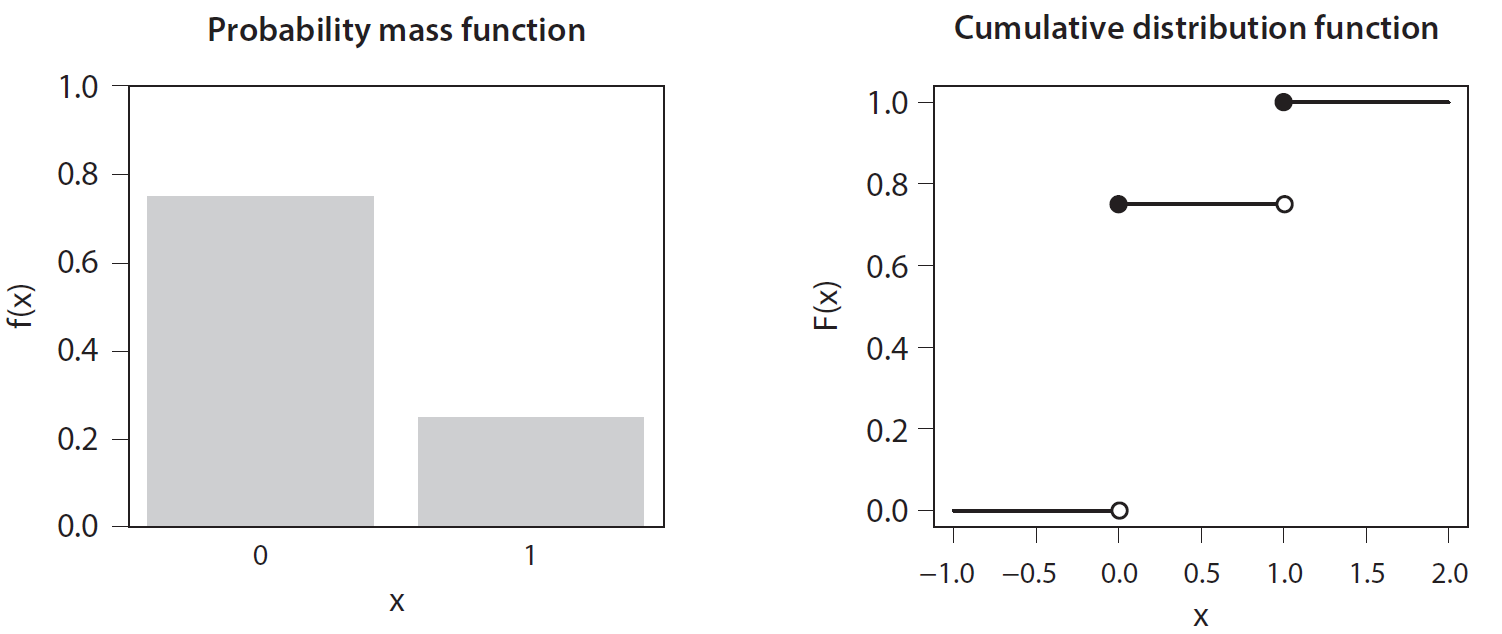
\includegraphics[scale=0.35]{../../LaTex/img/bernoulli_distribution.png}
    \end{center}
\end{frame}

\begin{frame}{Uniform Distribution. The simplest  continuous distribution}
    \begin{itemize}
        \item \textbf{Definition:} A continuous random variable with equal probability for all values in an interval \([a, b]\).
        \item \textbf{PDF} (\texttt{dunif()}):
        \[
        f(x) =
        \begin{cases}
        \frac{1}{b-a}, & \text{if } a \leq x \leq b \\
        0, & \text{otherwise}
        \end{cases}
        \]
        \item \textbf{Example:}
        \begin{itemize}
            \item[$\bullet$] Randomly choosing a point in \([0, 1]\).
        \end{itemize}
    \end{itemize}
\end{frame}

\begin{frame}{Visualization of the uniform distribution}
    \begin{center}
    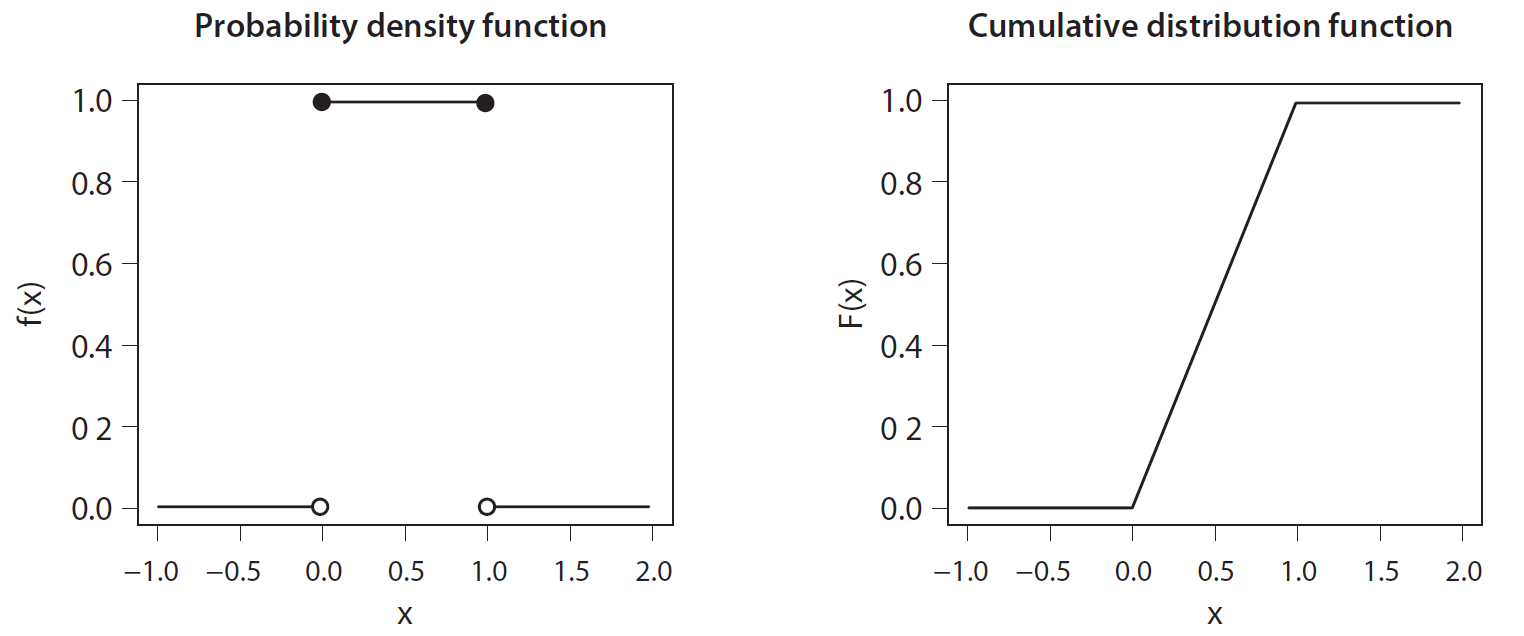
\includegraphics[scale=0.35]{../../LaTex/img/uniform_distribution.png}
    \end{center}
\end{frame}

\begin{frame}{Binomial Distribution}
    \begin{itemize}
        \item \textbf{Definition:} A binomial random variable \(X\) represents the number of successes in \(n\) \textbf{independent trials}, each with success probability \(p\).
        \item \textbf{Examples:}
        \begin{itemize}
            \item[$\bullet$] Number of heads in \(n\) coin flips.
            \item[$\bullet$] Number of votes for a candidate in an election.
        \end{itemize}
        \item \textbf{Properties:}
        \begin{itemize}
            \item[$\bullet$] \(X\) takes values from 0 to \(n\).
            \item[$\bullet$] \(X\) is the sum of \(n\) \textbf{independent Bernoulli} random variables.
        \end{itemize}
    \end{itemize}
\end{frame}

\begin{frame}{Visualization of the binomial distribution}
    \begin{center}
    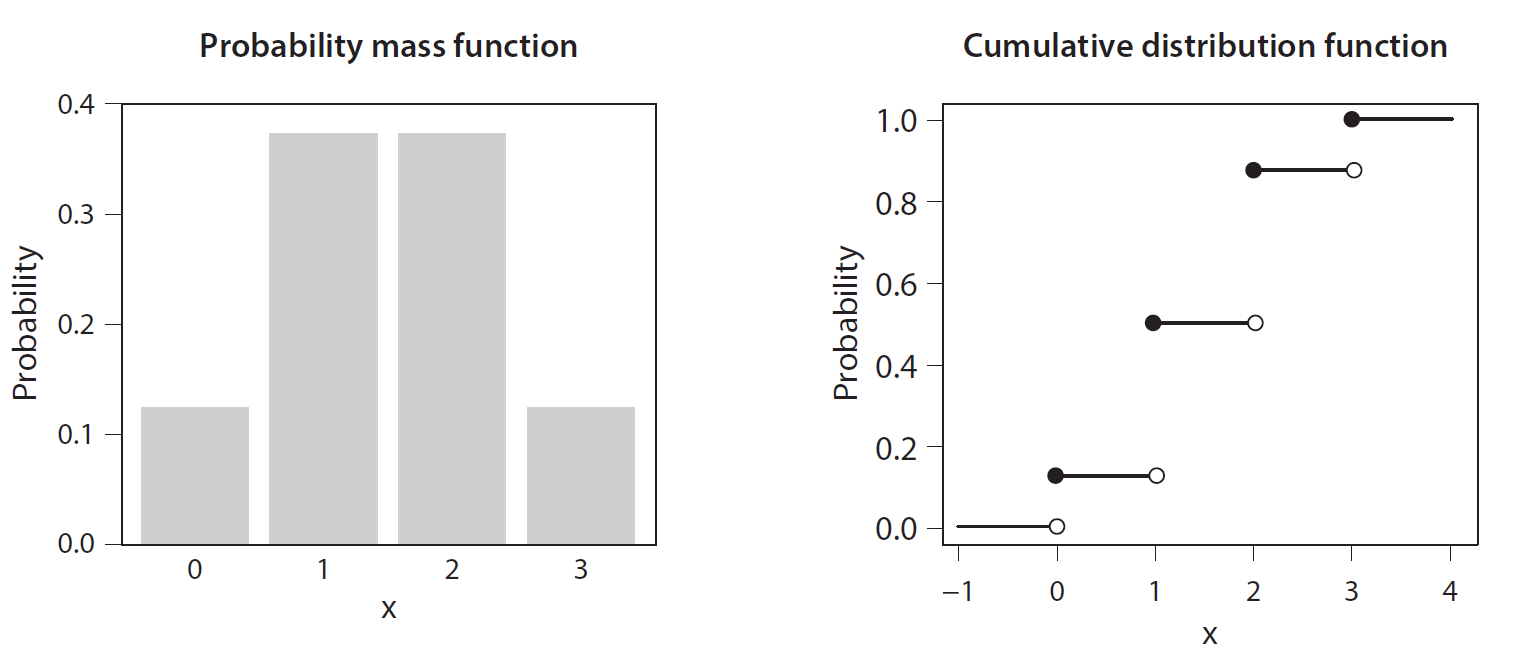
\includegraphics[scale=0.35]{../../LaTex/img/binomial_distribution.png}
    \end{center}
\end{frame}

\begin{frame}{Mass and distribution}
    \begin{itemize}
        \item \textbf{PMF} (\texttt{dbinom()}):
        \[
        P(X = x) = \binom{n}{x} p^x (1-p)^{n-x}, \quad x = 0, 1, \ldots, n
        \]
        \begin{itemize}
            \item[$\bullet$] \textbf{Recall:} \(\binom{n}{x} = \frac{n!}{x!(n-x)!}\) is the number of ways to choose \(x\) successes in \(n\) trials.
            \item[$\bullet$] \textbf{Example:} Probability of 2 successes in 3 independent trials with \(p = 0.5\):
            \[
            P(X = 2) = \binom{3}{2} 0.5^2 (1-0.5)^1 = 3 \cdot 0.25 \cdot 0.5 = 0.375
            \]
        \end{itemize}
        \item \textbf{CDF} (\texttt{pbinom()}):
        \[
        F(x) = P(X \leq x) = \sum_{k=0}^x \binom{n}{k} p^k (1-p)^{n-k}
        \]
        \begin{itemize}
            \item[$\bullet$] \textbf{Example:} Probability of at most 1 success in 3 trials with \(p = 0.5\):
            \[
            F(1) = P(X = 0) + P(X = 1) = 0.125 + 0.375 = 0.5
            \] 
        \end{itemize}
        
    \end{itemize}
\end{frame}

\begin{frame}{Application of Binomial Distribution}
    \begin{itemize}
        \item \textbf{Election Example:} Probability of a tie when $N$ voters turn out, each with $50\%$ support for a candidate:
        \[
        P(\text{Tie}) = P(X = 500), \quad X \sim \text{Binomial}(n=1000, p=0.5)
        \]
        \item \textbf{R code:} \\
        \texttt{\#\# number of voters who turn out \\
            voters <- c(1000, 10000, 100000) \\
            dbinom(voters / 2, size = voters, prob = 0.5) \\
            \#\# [1] 0.025225018 0.007978646 0.002523126
        }
    \end{itemize}
\end{frame}

\section{\large The normal distribution}

\begin{frame}{The Normal Distribution}
    \begin{itemize}
        \item Also known as the \textbf{Gaussian Distribution}.
        \item A continuous distribution over the real line $\R$.
        \item Characterized by two parameters:
        \begin{itemize}
            \item[$\bullet$] Mean (\(\mu\)): Center of the distribution.
            \item[$\bullet$] Standard deviation (\(\sigma\)): Controls the spread.
        \end{itemize}
        \item Notation: \(X \sim N(\mu, \sigma^2)\).
    \end{itemize}
\end{frame}

\begin{frame}{PDF and CDF}
    \begin{itemize}
        \item \textbf{PDF} (\texttt{dnorm()}):
        \[
        f(x) = \frac{1}{\sqrt{2\pi\sigma^2}} \exp\left(-\frac{(x - \mu)^2}{2\sigma^2}\right)
        \]
        \item \textbf{CDF:} (\texttt{pnorm()}):
        \[
        F(x) = P(X \leq x) = \int_{-\infty}^x f(t) \, dt, \quad \text{no explicit expression}
        \]
        \item Symmetric and bell-shaped, centered around \(\mu\).
        \item \(68\%\) of data lies within \(1\sigma\) of \(\mu\), and \(95\%\) within \(2\sigma\).
    \end{itemize}
\end{frame}

\begin{frame}{Visualization of the normal distribution}
    \begin{center}
    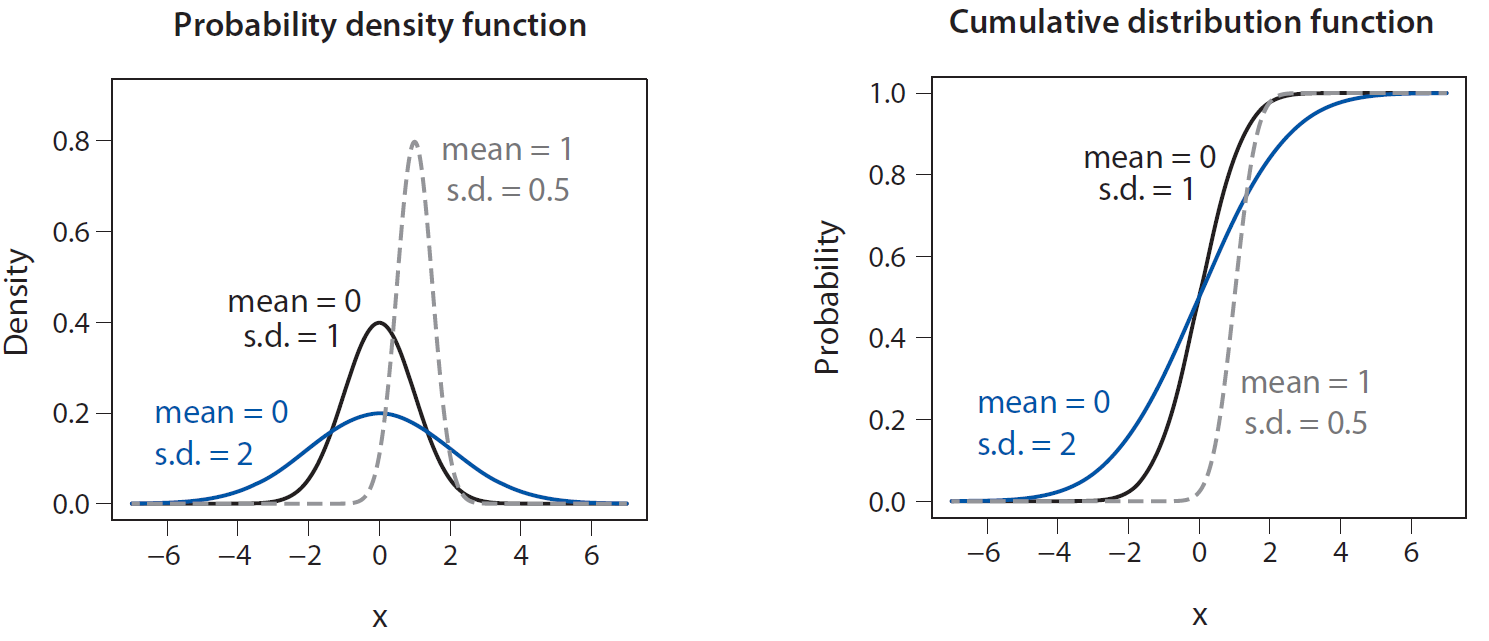
\includegraphics[scale=0.35]{../../LaTex/img/normal_distribution.png}
    \end{center}
\end{frame}

\begin{frame}{Properties of the Normal Distribution. Standardization}
    \begin{itemize}
        \item Suppose \(X \sim N(\mu, \sigma^2)\) is a normal random variable.
        \item For any constant \(c\), the following properties hold:
        \begin{enumerate}
            \item Adding \(c\) to \(X\):
            \[
            Z = X + c \implies Z \sim N(\mu + c, \sigma^2)
            \]
            \item Multiplying \(X\) by \(c\):
            \[
            Z = cX \implies Z \sim N(c\mu, (c\sigma)^2)
            \]
        \end{enumerate}
        \item \textbf{Z-score Transformation:}
        \[
        Z = \frac{X - \mu}{\sigma} \implies Z \sim N(0, 1)
        \]
        \item The \textbf{Z-score} standardizes \(X\) to have zero mean and unit variance.
        \item \textbf{Applications:}
        \begin{itemize}
            \item[$\bullet$] Standardizing data for comparison.
            \item[$\bullet$] Calculating probabilities using standard normal tables. \\ Useful back in the days but obsolete with the advent of programming languages.
        \end{itemize}
    \end{itemize}
\end{frame}

\begin{frame}{An application}

    \begin{itemize}
        \item Based on the 2008 and 2012 US election data, the following model is proposed
        \begin{align*}
            &\text{Obama’s 2012 standardized vote share} \\
            &\hspace{0.5cm} = 0.983 \times \text{Obama’s 2008 standardized vote share} + \epsilon, 
        \end{align*}        
        where $\epsilon\sim N(0, 0.18^2)$.
        \item In 2008, Obama won a standardized vote share of $0.87$ in California. What is the probability that Obama wins a greater share of California votes in 2012?
        \item In 2008, Obama won a standardized vote share of $-0.67$ in Texas. What is the probability that Obama wins a greater share of Texas votes in 2012?
        \item \textbf{R code:}
        \texttt{\\
            \# probability for California \\
            pnorm(0.87, mean = 0.983 * 0.87, sd = 0.18, lower.tail = FALSE) \\
            \# probability for Texas \\
            pnorm(-0.67, mean = 0.983 * -0.67, sd = 0.18, lower.tail = FALSE)
        }
    \end{itemize}
\end{frame}

\section{\large Expectation and Variance}

\begin{frame}{Expectation (Mean)}
    \begin{itemize}
        \item \textbf{Definition:} The theoretical average value of a random variable.
        \item For a random variable \(X\):
        \[
        E(X) =
        \begin{cases}
        \sum_x x f(x), & \text{if } X \text{ is discrete} \\
        \int_{-\infty}^\infty x f(x) \, dx, & \text{if } X \text{ is continuous}
        \end{cases}
        \]
        \item \textbf{Examples:}
        \begin{itemize}
            \item[$\bullet$] Bernoulli$(p)$: \(E(X) = p\)
            \item[$\bullet$] Binomial$(n, p)$: \(E(X) = np\)
            \item[$\bullet$] Uniform$[a, b]$: \(E(X) = \frac{a + b}{2}\)
        \end{itemize}
    \end{itemize}
\end{frame}

\begin{frame}{Variance and Standard Deviation}
    \begin{itemize}
        \item \textbf{Variance:} Measures the spread (from the mean) of a random variable.
        \[
        V(X) = E[(X - E(X))^2] = E(X^2) - (E(X))^2
        \]
        \item \textbf{Standard Deviation:} The square root of variance:
        \[
        \text{SD}(X) = \sqrt{V(X)}
        \]
        \item \textbf{Examples:}
        \begin{itemize}
            \item[$\bullet$] Bernoulli$(p)$: \(V(X) = p(1-p)\)
            \item[$\bullet$] Binomial$(n, p)$: \(V(X) = np(1-p)\)
            \item[$\bullet$] Uniform$[a, b]$: \(V(X) = \frac{(b-a)^2}{12}\)
        \end{itemize}
    \end{itemize}
\end{frame}

\begin{frame}{Properties of Expectation and Variance}
    \textbf{Expectation Rules:}
    \begin{itemize}
        \item \(E(a) = a\)
        \item \(E(aX) = aE(X)\)
        \item \(E(aX + bY) = aE(X) + bE(Y)\)
        \item For independent \(X\) and \(Y\): \(E(XY) = E(X)E(Y)\)
    \end{itemize}
    \vspace{0.5cm}
    \textbf{Variance Rules:}
    \begin{itemize}
        \item \(V(aX) = a^2V(X)\)
        \item \(V(X + b) = V(X)\)
        \item For independent \(X\) and \(Y\): \(V(X + Y) = V(X) + V(Y)\)
    \end{itemize}
\end{frame}

\section{\large Large Sample Theorems}

\begin{frame}{Law of Large Numbers, a.k.a. ``The Wisdom of the Crowd''}
    \begin{itemize}
        \item In 1906, the statistician Francis Galton\footnote{The same statistician who ran the first recorded experiment of linear regression} observed a competition of eight hundred people trying to guess the weight of an ox at a country fair. 
        
        \item \href{https://www.nature.com/articles/075450a0.pdf}{He discovered} that the average guess (1,197lb) was extremely close to the actual weight (1,198lb).
        
        \item This illustrates the Law of Large Numbers (LLN): as the number of observations increases, the sample mean approaches the true mean.
    \end{itemize}
\end{frame}

\begin{frame}{Law of Large Numbers (LLN)}
    \begin{itemize}
        \item \textbf{Definition:} As the sample size (\(n\)) increases, the sample average (\(\bar{X}\)) converges to the population mean (\(E(X)\)):
        \[
        \bar{X}_n = \frac{1}{n} \sum_{i=1}^n X_i \xrightarrow[n\rightarrow\infty]{}  E(X).
        \]
        \item \textbf{Key Idea:} The sample mean becomes a better approximation of the true mean as \(n\) grows.
        \item \textbf{Applications:}
        \begin{itemize}
            \item Survey results approximate population opinions.
            \item Simulations approximate theoretical probabilities.
            \item \href{https://en.wikipedia.org/wiki/Condorcet's_jury_theorem}{Condorcet’s Jury Theorem}: when certain assumptions hold, the probability that a majority of voters support the correct decision increases and approaches one as the number of voters increases
        \end{itemize}
    \end{itemize}
\end{frame}

\begin{frame}{Illustrating LLN}
    \textbf{R code:}\\
    \texttt{n <- 1000 \# number of simulations \\ 
        x.binom <- rbinom(n, p = 0.2, size = 10) \# simulating\\
        mean.binom <- cumsum(x.binom) / 1:n \# computing sample mean\\
        plot(1:1000, mean.binom, type = "l", ylim = c(1, 3), xlab = "Sample size", \\
        \hspace{0.87cm} ylab = "Sample mean", main = "Binomial(10, 0.2)") \\ 
        abline(h = 2, lty = "dashed") \# expectation
        }     
        \vspace{-0.1cm}
        
        \begin{minipage}{0.4\textwidth}
            \begin{itemize}
                \item Simulating \(n = 1000\) draws from a Binomial(10, 0.2).
                \item Sample mean (\(\bar{X}\)) approaches the expectation \(E(X) = 2\).
            \end{itemize}
        \end{minipage}
        \hspace{0.5cm}
        \begin{minipage}{0.55\textwidth}
            \begin{center}
                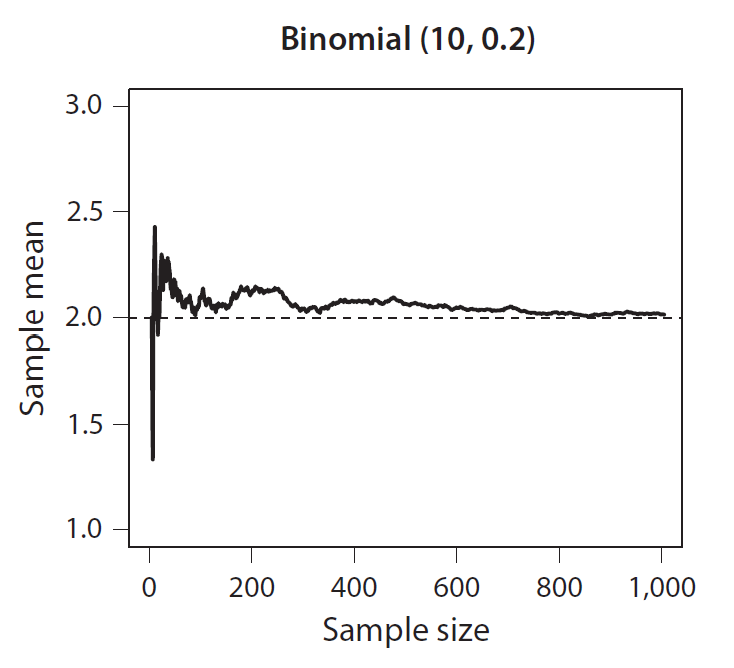
\includegraphics[width=0.9\textwidth, height = 4.5cm]{../../LaTex/img/LLN.png}    
            \end{center}
        \end{minipage}
\end{frame}

\begin{frame}{Central Limit Theorem (CLT)}
    \begin{itemize}
        \item \textbf{Definition:} The sample mean (\(\bar{X}_n\)) of \(n\) independent, identically distributed (i.i.d.) observations converges in distribution to a normal distribution as \(n\) increases:
        \[
        Z = \frac{\bar{X}_n - E(X)}{\sqrt{V(X)/n}} \approx N(0, 1)
        \]
        \item \textbf{Key Idea:} Regardless of the original distribution, the sample mean’s distribution becomes approximately normal for large \(n\).
        \item \textbf{Applications:}
        \begin{itemize}
            \item Estimating error for sample means.
            \item Understanding variability in data collection.
        \end{itemize}
    \end{itemize}
\end{frame}

\begin{frame}{Illustrating CLT}
    \begin{itemize}
        \item Simulate Z-scores for \(n = 1000\).
        \item Sample mean’s z-scores follows \(N(0, 1)\) distribution.
    \end{itemize}
    \vspace{0.1cm}
    
    \begin{center}
        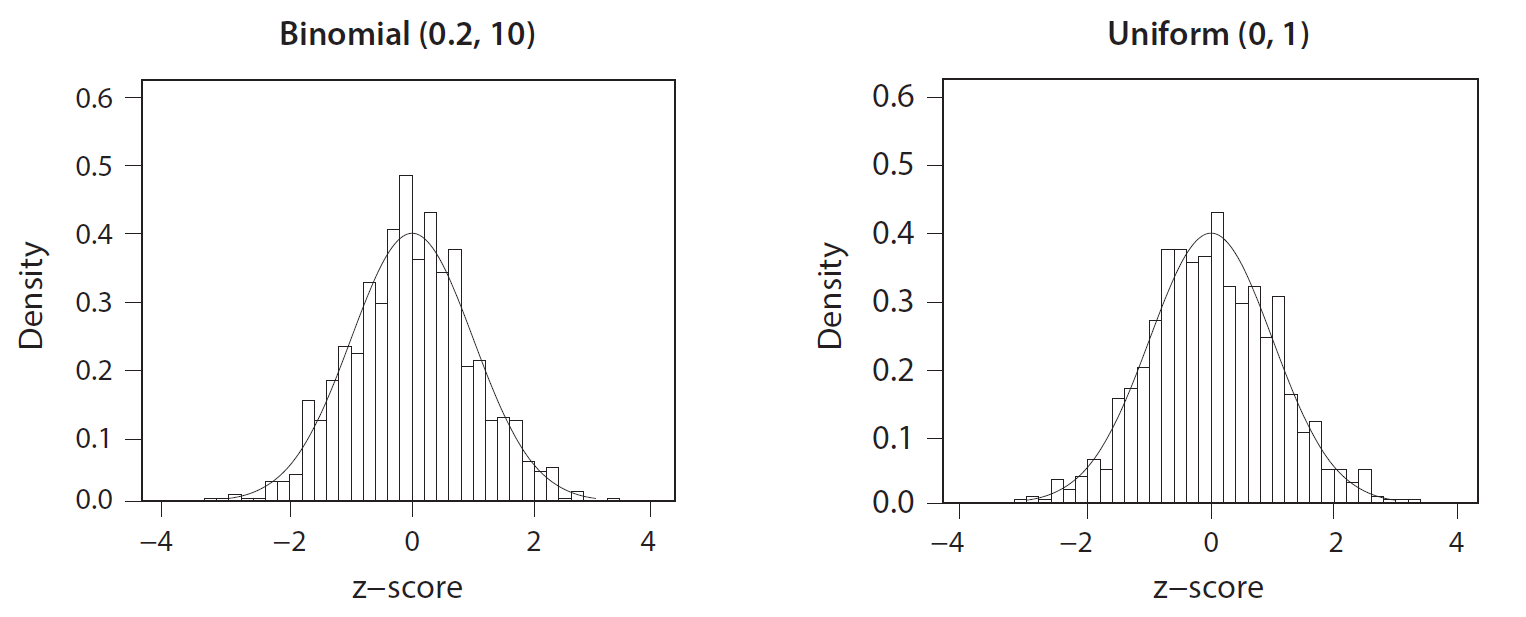
\includegraphics[width=0.9\textwidth]{../../LaTex/img/CLT.png}    
    \end{center}
\end{frame}

\end{document}
